\section{Auswertung}
\label{sec:Auswertung}

Im folgenden werden die Daten analysiert, die während einer Messzeit von ungefähr $T_{Messung} = 5  \unit\day$ aufgenommen wurden.

\subsection{Kalibrierung der Messgeräte}

Bei der Kalibrierung der Geräte trat ein Problem bei der Einstellung der Pulsdauer auf.
Aus diesem Grund wurde die Pulsdauer statt auf $10 \unit{\nano\second}$ auf $20 \unit{\nano\second}$ und $30 \unit{\nano\second}$ eingestellt.
Die Messdaten dazu sind in \autoref{tab:20ns_table} und \autoref{tab:30ns_table} zu finden.
Die Plots der Daten und der entsprechenden Halbwertsbreiten sind in \autoref{fig:20ns_plot} und \autoref{fig:30ns_plot} zu finden.
Für eine Pulsdauer von $20 \unit{\nano\second}$ ergibt sich eine Halbwertsbreite von $\Delta_\text{Breite} = 25 \unit{\nano\second}$, woraus sich dann eine Verzögerung von
\begin{equation*}
    (2 \cdot 20 - 25) \unit{\nano\second} = 15 \unit{\nano\second}  
\end{equation*}
ergibt.
Für eine Pulsdauer von $30 \unit{\nano\second}$ ergibt sich eine Halbwertsbreite von $\Delta_\text{Breite} = 37 \unit{\nano\second}$, woraus sich dann eine Verzögerung von
\begin{equation*}
    (2 \cdot 30 - 37) \unit{\nano\second} = 23 \unit{\nano\second}  
\end{equation*}
ergibt.
\input{build/20ns_table.txt}
\input{build/30ns_table.txt}


\begin{figure}
    \centering
    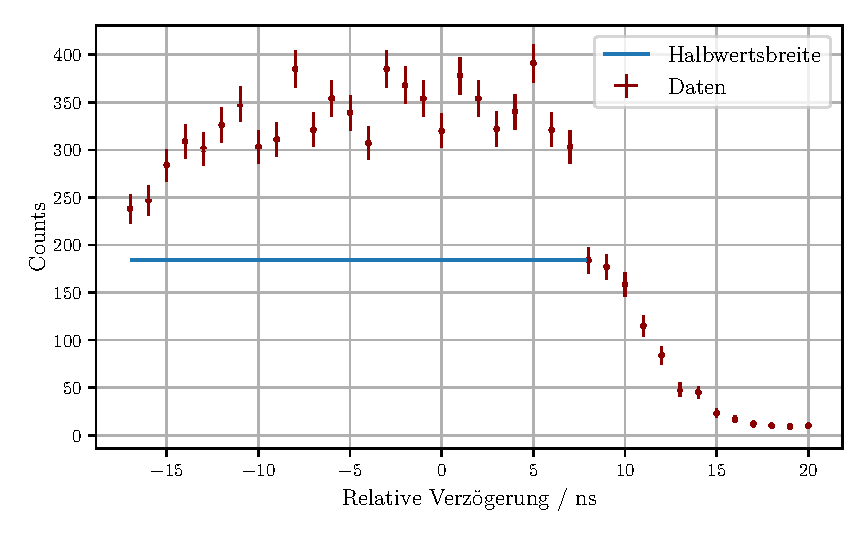
\includegraphics[width = 0.7 \linewidth]{build/20ns_plot.pdf}
    \caption{Plot zur Messung bei einer Pulsdauer von $20$ns.}
    \label{fig:20ns_plot}
\end{figure}


\begin{figure}
    \centering
    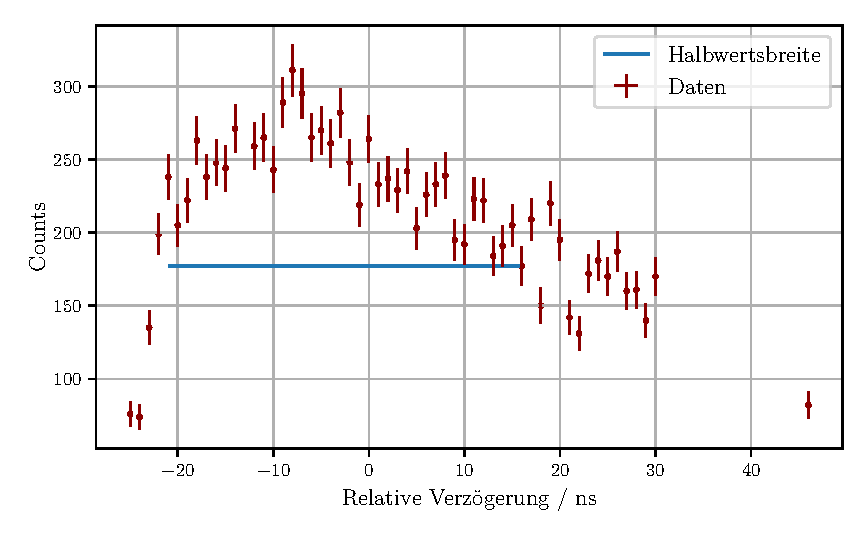
\includegraphics[width = 0.7 \linewidth]{build/30ns_plot.pdf}
    \caption{Plot zur Messung bei einer Pulsdauer von $30$ns.}
    \label{fig:30ns_plot}
\end{figure}

\subsection{Bestimmung der Zeiteinteilung der Bins am TCA}

Die Messdaten sind in \autoref{tab:zeiteinteilung} zu finden.
Um den Bins des TCAs eine Zeit zuzuordnen, wird eine Regressionsrechnung durchgeführt.
Dafür wird der Ansatz
\begin{equation*}
    t = m \cdot x + b
\end{equation*}
gewählt.
Der entsprechende Plot st in \autoref{fig:zeiteinteilung} abgebildet.
Der Fit ergibt $m = 0.02257 \pm 0.00005$ und $b = 0.148 \pm 0.006$

\begin{figure}
    \centering
    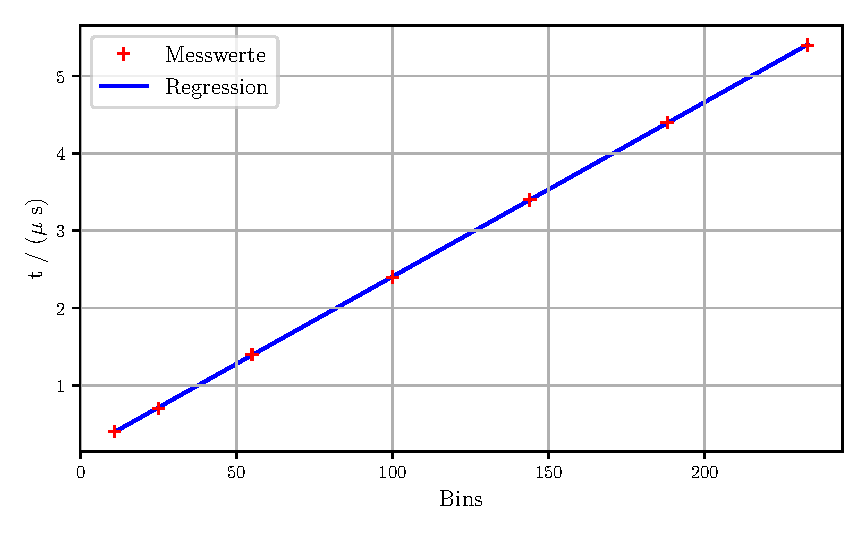
\includegraphics[width = 0.7 \linewidth]{build/zeiteinteilung.pdf}
    \caption{Bestimmung der zeiteinteilung der Bins.}
    \label{fig:zeiteinteilung}
\end{figure}

\input{build/zeiteinteilung.txt}